\section{Programmazione concorrente}

Un programma concorrente dispone di due o più flussi di esecuzione contemporanei,
per perseguire un obiettivo comune probabilmente in un tempo inferiore.

Tali flussi possono essere eseguiti in
parallelo (se il processore dispone di più core) e/o alternarsi nel tempo, sotto
il controllo di uno schedulatore.

All'atto della creazione, un processo dispone di un \textbf{unico flusso di esecuzione},
il thread principale, che esegue il codice del programma, il quale può
chiedere allo schedulatore di creare nuovi thread.

Un thread rappresenta una \textbf{computazione indipendente}.

Basata su un proprio stack (pre-allocato all'atto della creazione del thread)
collocato nello stesso spazio di indirizzamento in cui operano gli altri thread
del processo. Tale computazione si svolge fino al proprio termine, potendo dare
origine ad un \textbf{risultato} o ad un errore, provocando un \textbf{abort}.

Il S.O. e/o le librerie di supporto allocano le risorse fisiche necessarie,
lo scheduler ripartisce, nel tempo, l'utilizzo dei core disponibili tra i
diversi thread in modo non deterministico. Tutti i thread creati sono
identificati in modo univoco e viene mantenuto, per quelli in uso, l'indicazione
del loro stato di esecuzione.

La gestione dei thread può essere demandata direttamente al S.O., in questo caso
si parla di \textbf{thread nativi}, oppure gestita da librerie a livello utente,
con il supporto parziale del sistema operativo.
Questi vengono detti \textbf{green thread} o \textbf{fibre} e richiedono una
certa forma di cooperazione da parte del codice che deve, in modo esplicito,
invocare lo scheduler per cedere l'uso della CPU.

C++ e Rust offrono, nella propria libreria standard, supporto per i thread nativi,
inoltre, entrambi offrono librerie di terze parti per il supporto di green thread
nascondendo i dettagli implementativi.

\section{Thread nativi}

I diversi sistemi operativi offrono funzionalità simili, ma non identiche, per
governare l'interazione di un programma con l'insieme dei thread che lo
costituiscono

Le funzioni supportate da tutti i sistemi operativi sono:

\begin{itemize}
  \item \textbf{Creazione}: di un thread, indicando la funzione che
        rappresenta la computazione che deve essere svolta e la dimensione dello stack
        richiesto: questa operazione restituisce un \textbf{handle} opaco mediante il quale
        fare riferimento al thread
  \item \textbf{Identificazione}: del thread corrente, sotto forma di valore
        univoco a livello di sistema (TID - Thread ID)
  \item \textbf{Attesa}: della terminazione di un thread, a partire dalla sua
        handle, e accesso al suo stato finale, successo/fallimento.
\end{itemize}

Tra le funzioni non supportate, spiccala richeista di \textbf{cancellazione} di un thread.
Questa può solo essere implementata in modo cooperativo dal thread stesso.
Per farli terminare sta al programmatore a scrivere del codice che li faccia
terminare.

\subsection{Processi, thread e modelli di esecuzione}

\begin{table}[h!]
  \renewcommand{\arraystretch}{1.6}
  \centering
  \begin{tabularx}{0.7\textwidth}{X X X}
    \toprule
    \textbf{Entità}      & \textbf{Memoria}                                          & \textbf{Gestione}  \\
    \midrule
    Processo             & Spazio di indirizzamento proprio                          & Sistema operativo  \\
    Thread nativo        & stack proprio, heap/variabili globali/codice condivisi    & Sistema operativo  \\
    Green thread / Fibra & Possono, come no, avere uno stack. Nel processo ospitante & Libreria / runtime \\
    \bottomrule
  \end{tabularx}
\end{table}

\begin{tcolorbox}
  \textbf{Nota:} Più thread nello stesso processo condividono i dati, ma non lo stack
\end{tcolorbox}


Nei processi, nei sistemi Unix, la crazione di un nuovo processo con \textbf{fork},
si crea una copia completa dello spazio di indirizzamento del processo padre,
rendedo difficile la comunicazione tra i processi, che avviene tramite meccanismi di
IPC (Inter Process Communication).

Il concetto di thread, ovvero condividere lo spazio di indirizzamento tra più flussi
di esecuzione, introduce molte insidie.

\subsection{Cosa implica la concorrenza}
Ad inizio degli anni 2000, era difficile scrivere programmi concorrenti perché
non esistevano strumenti per gestire la multipiattaforma, fino a che l'uscita
di Java, con il suo supporto nativo per i thread e multipiattaforma.
Il C++ solo nel 2011, 13 anni dopo Java, ha introdotto questo supporto mancate.


Possibilità di \textbf{sovrapporre temporalmente} attività di computazione e
operazioni di I/O:

\begin{itemize}
  \item I sistemi operativi tendono ad offrire API bloccanti che arrestano, di fatto, la prosecuzione di un
        thread fino a che il dato richiesto non è pronto (es.: read(fd), accept(socket), …)
  \item  Suddividendo l'algoritmo in più thread, si può cercare sfruttare i tempi di attesa che un dato thread
        subisce a seguito delle operazioni di I/O per eseguire, in altri thread, operazioni utili al risultato
  \item  Occorre che la complessità aggiunta dalla suddivisione sia compensata da un effettivo guadagno in
        termini di tempi di esecuzione
\end{itemize}


Ci sono molti motivi per utilizzare i thread, tra cui efficientare e utilizzare
al meglio le risorse hardware che abbiamo a disposizione. Sfruttando
i momenti morti, come l'I/O, per eseguire altre operazioni.


\textbf{Riduzione del sovraccarico} dovuto alla comunicazione tra processi

\begin{itemize}
  \item  Sebbene la suddetta parallelizzazione possa essere fatta anche creando processi separati, il costo di
        comunicazione e sincronizzazione tra processi è sensibilmente più alto di quello tra thread
  \item I thread condividono infatti lo spazio di indirizzamento: questo rende più efficiente la condivisione dei
        dati rispetto a processi distinti
  \item Tale efficienza \textbf{non implica sicurezza} automatica: gli accessi conocrrenti ai
        dati condivisi richiedono \textbf{sincronizzazione}
\end{itemize}

Potrei creare dure processi distinti, ma durante il merge dei dati porta ad una serializzazione
di dati che potrebbe essere più costosa.
Lo spazio di indirizzamento tra thread è condiviso, sia nel bene che nel male.

\begin{itemize}
  \item Possibilità di sfruttare appieno le capacità di \textbf{elaborazione} delle CPU
        \textbf{multicore}. Più flussi di esecuzione possono svolgersi contemporaneamente,
        riducendo così il tempo totale di elaborazione: vero parallelismo
  \item \textbf{Aumento} significativo \textbf{della complessità} del programma. Nuove fonti e
        tipologie di errore. \textbf{Non determinismo dell'esecuzione}, non risucendo a definire
        a livello di sistema operativo l'ordine di esecuzione dei thread.
  \item La memoria \textbf{non} può più essere pensata come un ``\textbf{deposito statico}''. I
        dati scritti al suo interno possono cambiare in conseguenza dell'attività di
        altri thread
  \item I thread devono \textbf{coordinare l'accesso} alla memoria. Tramite opportuni
        costrutti di sincronizzazione. La presenza di cache legate ai singoli core
        introduce non determinismo nell'ordinamento e nella visibilità delle azioni
        sulla memoria
\end{itemize}

\subsection{Concorrente e parallelismo}

\paragraph{Concorrente} più flussi di elaborazione \textbf{attivi} nello stesso
intervallo di tempo, il cui avanzamento può avvenire. In alternanza su uno
stesso core sotto il controllo dello scheduler. Oppure in parallelo se sono
disponibili più core.

\paragraph{Parallelismo} caso particolare in cui i flussi di elaborazione sono
realmente in esecuzione nello stesso istante. Perché assegnati a core distinti

\begin{tcolorbox}
  \textbf{Nota}:  Ogni parallelismo è una forma di concorrenza,ma non ogni
  concorrenza implica parallelismo
\end{tcolorbox}

\subsection{Concorrenza in pratica}

Se, all'interno di un processo, sono presenti due o più thread, questi possono
procedere indipendentemente nella propria computazione. Sebbene sia possibile
creare thread che si ignorano reciprocamente e non necessitano alcuno scambio di
informazione, sul piano pratico questo avviene molto raramente.

L'utilità di
suddividere la computazione globale in più sotto-computazioni nasce, per lo più,
dal fatto che ciascuna di esse contribuisce in qualche modo al risultato finale. Questo richiede che esista una forma di comunicazione/sincronizzazione tra
thread differenti.

I meccanismi soggiacenti alla comunicazione/sincronizzazione
interferiscono con le ottimizzazioni usate dai processori per migliorare
l'esecuzione. Introducendo una serie di \textbf{complessità inattese} e lontane dal
pensiero comune legato al modello di esecuzione sequenziale.

\paragraph{}

In un sistema single-core, il concetto di thread è puramente una astrazione
offerta dal sistema operativo. Il processore si limita ad alternare il proprio
ciclo di esecuzione basato sulla successione delle microoperazioni
\textbf{fetch/decode/execute}, procedendo di istruzione in istruzione secondo la logica
del codice macchina.

Il sistema operativo può intervenire in questa sequenza, grazie ad
un'interruzione che attiva lo scheduler. Questo salva lo stato dei registri in
una qualche area di memoria dedicata alle meta-informazioni del thread corrente
e li ripristina con il contenuto relativo ad un thread differente, \textbf{task
  switching}.


Se la CPU è dotata di due o più core, non cambia molto. Ciascun core procede
indipendentemente dagli altri e lo scheduler provvede a gestire le attività di
tutti, allocando di volta in volta i core disponibili ad eseguire l'uno o
l'altro thread, secondo le necessità.


\paragraph{}

Poiché l'esecuzione di ciascun thread procede indipendentemente da quelle degli
altri, un'eventuale necessità di comunicazione deve essere soddisfatta passando
per l'utilizzo di un'area di memoria condivisa. In cui il thread T1 possa
depositare le informazioni che intende comunicare al thread T2.

Sebbene i due
thread utilizzino lo stesso spazio di indirizzamento e possano, in linea di
principio, accedere al dato memorizzato, questa operazione risulta \textbf{più complessa}
di quanto si possa pensare a prima vista. Per rendere la comunicazione utile
sul piano pratico, può essere inoltre necessario avvalersi di pattern di
interazione che definiscano con precisione i ruoli che le due o più parti
coinvolte possono giocare.



\section{Modello di memoria}

Quando un thread legge il contenuto di una locazione di memoria, può trovare:

\begin{itemize}
  \item Il valore iniziale contenuto nel file eseguibile che è stato mappato in memoria (es: variabile globale
        inizializzata)
  \item Il valore che questo stesso thread ha precedentemente depositato all'interno della locazione
  \item Il valore che è stato depositato da un altro thread
\end{itemize}
La presenza di cache hardware e il possibile riordinamento delle istruzioni da parte
della CPU rendono il terzo caso problematico. In generale non è predicibile quale valore venga letto senza controllare letture e scritture da parte dei
thread. Occorre usare un costrutto di sincronizzazione esplicito che permetta di definire l'ordine di esecuzione

\begin{center}
  \begin{minipage}{0.47\linewidth}
    \centering
    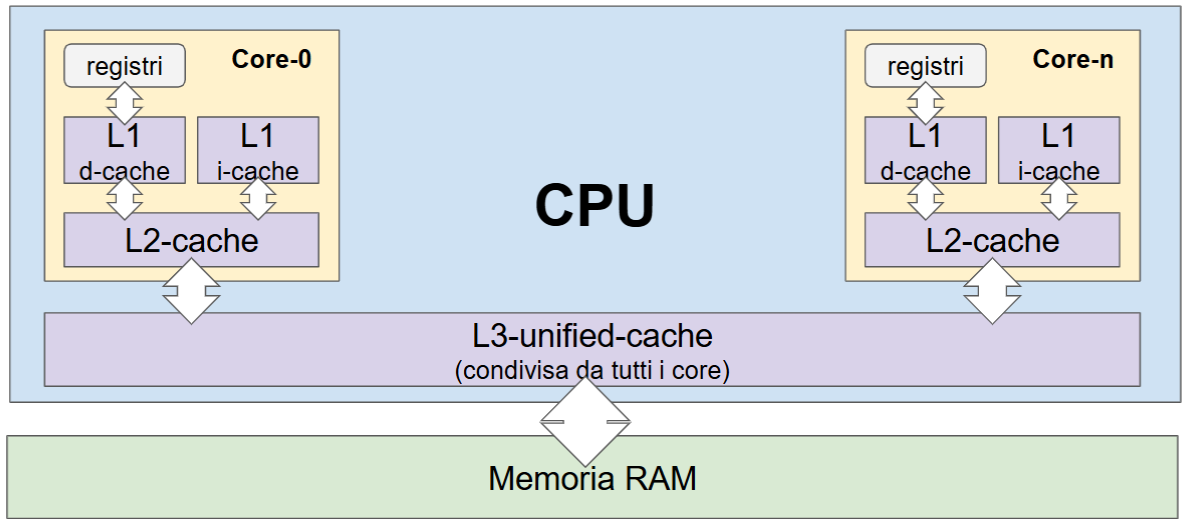
\includegraphics[width=\linewidth]{content/API_Programming/images/2026-04-27-12-27-32.png}
  \end{minipage}%
  \hfill
  \begin{minipage}{0.47\linewidth}
    \centering
    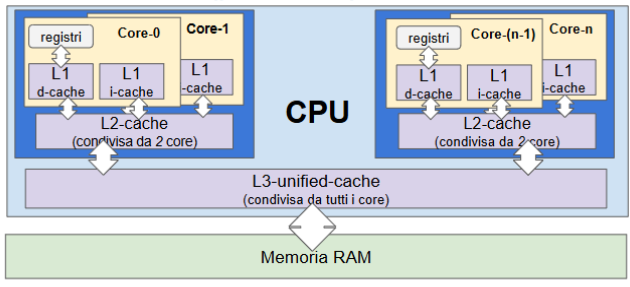
\includegraphics[width=\linewidth]{content/API_Programming/images/2026-04-27-12-28-33.png}
  \end{minipage}
\end{center}


\subsection{Problemi aperti}
La cache porta con se un problema, ogni thread agisce sulla propria cache, se vogliamo che i
dati fluiscano tra una cache e l'altra occorre tempo.

Sorgono 3 problemi, in un contesto sequenziale non è presente:

\begin{itemize}
  \item\textbf{Atomicità}: Solitamente vogliamo salvare più di un byte alla volta. Non è detto che quella operazione stia perfettamente in una riga di cache.
  \item \textbf{Visibilità}: Ogni thread scrive sulla propria cache, e se forzo il sync della cache solo a quel punto i dati sono visibili a tutti
  \item \textbf{Ordinamento}: La sequenza, dato il tempo di re-sync, non è garantito e l'ordine dei risultati non è predicibile
\end{itemize}


La cache è un fatto puramente Hardware, in nessun linguaggio di programma, se pur a basso livello come ARM,
non è possibile accedere direttamente alla cache.
Il processore non ha consapevolezza che ha una cache.


\begin{table}[h!]
  \renewcommand{\arraystretch}{1.6}
  \centering
  \begin{tabularx}{0.8\textwidth}{l X X}
    \toprule
    \textbf{Problema} & \textbf{Domanda chiave}                                             & \textbf{Esempio intuitivo}                                                           \\
    \midrule
    Atomicità         & L'operazione è atomica?                                             & a += 1 consiste in una lettira seguita da una scrittura, 3 operazioni, non è atomica \\
    Visibilità        & Un altro thread vede davvero la scrittura?                          & Un thread legge un valore obsoleto                                                   \\
    Ordinamento       & Gli altri thread osservano operazioni distinte nello stesso ordine? & Scritture viste in un ordine diverso                                                 \\
    \bottomrule
  \end{tabularx}
\end{table}

\section{La risposta dei processori}

Ciascuna famiglia di processori offre una propria risposta ai problemi menzionati.

La piattaforma \textbf{x86} adotta un modello \textbf{quasi sequenzialmente consistente} ed offre
le istruzioni di tipo fence, che forzano il completamento delle operazioni di
scrittura, bloccando temporaneamente gli altri core che dovessero cercare di
accedere nel frattempo allo stesso segmento di indirizzi

Per contro, sulla
piattaforma \textbf{ARM} viene usato un modello molto più lasco, basato su \textbf{liste di
  propagazione dei cambiamenti}, ed offre le istruzioni di tipo barrier che
consentono l'ordinamento causale rispettivamente per il calcolo degli indirizzi,
delle istruzioni, dei dati.


Se tali istruzioni non vengono incluse all'interno del codice generato, \textbf{non è
  garantito un ordinamento predicibile}, quando due thread diversi, alle operazioni di \textbf{lettura e scrittura di
  dati condivisi}, in presenza di attività concorrenti.
C++ e Rust condividono il
modello di memoria su cui sono basati e annegano, nelle funzioni di libreria dei
tipi dedicati alla concorrenza, tali istruzioni allo scopo di garantire le
necessarie proprietà di funzionamento



\subsection{Errori comuni}

\begin{itemize}
  \item L'\textbf{uso superficiale} dei costrutti di sincronizzazione porta a blocchi
        passivi o attivi del programma. In ogni caso, fonte di guai per il
        programmatore
  \item L'\textbf{assenza} di costrutti di sincronizzazione, porta a risultati
        imprevedibili. Anche molto lontani da quanto sarebbe logico aspettarsi
  \item Si possono verificare \textbf{malfunzionamenti casuali}: Dovuti al
        comportamento non deterministico e asincrono dell'esecuzione concorrente.
        Estremamente difficili da riprodurre e da eliminare
  \item Gli errori possono manifestarsi cambiando la \textbf{piattaforma di esecuzione}, oppure
        Oppure soltanto dopo numerose esecuzioni. Tipicamente emergono nel momento
        meno adatto.
\end{itemize}


\section{Thread e memoria}



\begin{flushleft}
  \begin{minipage}{0.65\linewidth}
    \raggedright
    Il sistema operativo mantiene, al proprio interno, una rappresentazione dei thread
    presenti all'interno di un dato processo.
    Ad ogni thread viene associato un identificativo univoco (TID - Thread ID), il suo stato di esecuzione
    (non schedulabile, schedulabile, in esecuzione sul core i, terminato con errore, terminato senza
    errore, …) e le informazioni necessarie a salvare/ripristinare lo stato dei registri interni al processore.
    Provvede inoltre ad allocare, nello spazio di indirizzamento del processo, un blocco di indirizzi contigui
    destinato ad ospitare lo stack che governerà la sua esecuzione


    Tutti i thread presenti in un processo condividono:

    \begin{itemize}
      \item Le variabili globali
      \item Le costanti
      \item L'area eseguibile in cui è contenuto il codice
      \item Lo heap
    \end{itemize}
  \end{minipage}%
  \hfill
  \begin{minipage}{0.3\linewidth}
    \centering
    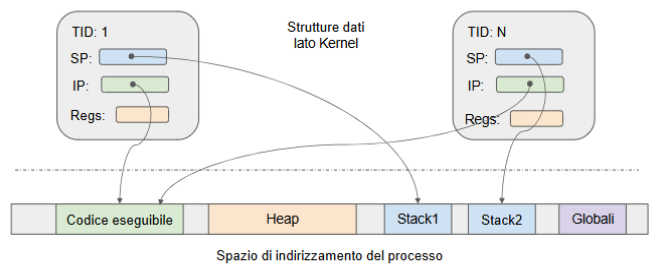
\includegraphics[width=\linewidth]{content/API_Programming/images/2026-04-27-12-58-10.png}
  \end{minipage}
\end{flushleft}

\subsection{Esecuzione e non determinismo}


\begin{itemize}
  \item  L'esecuzione di ogni singolo thread procede secondo le normali regole sequenziali. Per cui è possibile prevedere cosa avvenga "prima" e cosa "dopo"
  \item Se più thread sono in esecuzione, non è possibile fare assunzioni sulle velocità relative di
        avanzamento. Se non ricorrendo a forme esplicite di sincronizzazione e comunicazione
  \item  La sincronizzazione può riguardare il raggiungimento di un particolare stato da parte di un
        thread.. Abilitando di conseguenza altri a procedere
  \item  ...oppure l'esigenza di un thread di eseguire azioni su aree condivise. Allo scopo di impedire ad altri di accedere alle stesse aree
  \item  In alcuni casi, all'informazione logica che abilita/impedisce la prosecuzione di altri thread,
        si accompagna il trasferimento di informazioni più strutturate. Che rappresentano l'esito totale o parziale di una computazione avvenuta o la richiesta di elaborazione di
        ulteriori dati
\end{itemize}


\begin{center}
  \begin{minipage}{0.75\linewidth}
    \begin{minted}[breaklines]{rust}
use std::thread;
use std::time::Duration;

fn run(msg: &str) {
  for i in 0..10 {
    println!("{}{}",msg,i);
    thread::sleep(Duration::from_nanos(1));
  }
  }
fn main() {
  let t1 = thread::spawn(|| {run( "aaaa"); });
  let t2 = thread::spawn(|| {run(" bbbb"); });
  t1.join().unwrap(); //uso di unwrap perché ritengo che non fallisca
  t2.join().unwrap();
  // sicuramente saranno stampati i vari aaaa e bbbb ma non possiamo dire l'ordine
}
\end{minted}
  \end{minipage}%
  \hfill
  \begin{minipage}{0.2\linewidth}
    \centering
    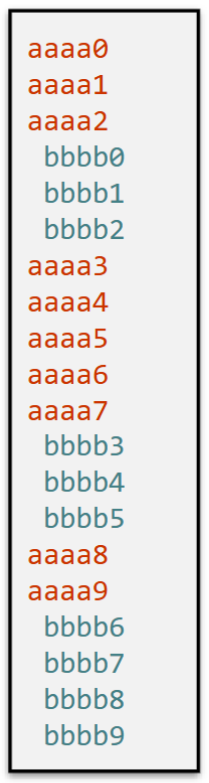
\includegraphics[width=0.5\linewidth]{content/API_Programming/images/2026-04-27-13-01-08.png}
  \end{minipage}
\end{center}

\section{Esecuzione e non determinismo}

\begin{itemize}
  \item L'output dei programmi precedenti è \textbf{solo uno}
\end{itemize}

\begin{minted}[breaklines]{rust}
#include <iostream>
#include <thread>
int a = 0; //Questo non è possibile in safe RUST
void run() {
  while (a >= 0) {
    int before = a;
    a++;  //il delta negativo è dato da questa operazione (non è atomica)
    int after = a;

    //in un contesto sequenzale, non passerebbe mai
    if (after-before != 1)
      std::cout << before << " -> " << after
      << "(" << after-before << ")\n";
  }
}

//creo due thread e ne attendo la terminazione
int main() {
  std::thread t1(run);
  std::thread t2(run);
  t1.join();
  t2.join();
}
\end{minted}


Esaminando l'uscita del programma precedente, si vedono molti casi in cui la
differenza tra \textbf{after} e \textbf{before} è superiore a \textbf{1}. In alcuni casi tale valore è
anche molto grande: perché?
Talora capita che la differenza sia \textbf{nulla}.
\textbf{negativa}. Come è possibile, se entrambi i flussi incrementano sempre la
variabile \textbf{a}?

\subsection{Interferenza}

\section{Sincronizzazione}

Se due thread cercano di accedere in lettura/scrittura ad una stessa variabile
si verifica una corsa critica, \textbf{race condition}.
In base a condizioni non controllabili dal programmatore (come la presenza di memoria cache, il
momento in cui avviene un task switch, le ottimizzazioni fatte dai singoli processori con la predizione
della prossima istruzione da eseguire, ...) il dato memorizzato potrebbe essere quello scritto dal primo
thread, quello scritto dal secondo oppure un terzo valore \textbf{completamente arbitrario}


L'accesso in lettura/scrittura a variabili il cui contenuto è (potenzialmente)
scritto da altri thread è soggetto a diversi vincoli:

\begin{itemize}
  \item Deve essere preceduto/seguito da istruzioni e proteggano da dati obsoleti presenti nella cache
        (fence/barrier)
  \item Deve avvenire solo quando c'è l'evidenza che il dato non sta venendo modificato da altri
  \item Se si sta operando una lettura in attesa di un risultato, si vuole evitare di eseguire cicli continui di
        polling, che consumano inutilmente cicli di CPU e batteria
\end{itemize}


Alcune delle condizioni citate sono garantite da \textbf{apposite istruzioni macchina}.
Che dipendono dal processore responsabile dell'esecuzione del codice.


Altre richiedono la garanzia di \textbf{invarianti a livello sistema} che può essere
fornita solo da meccanismi offerti dal sistema operativo. Che, controllando la
schedulazione dei thread, può farsi carico che avvenga / non avvenga una
determinata condizione.

Che sono i tipi atomici, i mutex operano su una struttura grande a piacere, e se dobbiamo aspettare
una codizione particolare ci sono le \textbf{condition mutex} utilizzabili assieme ad un mutex.

Ne consegue che i meccanismi di sincronizzazione dipendono dalla coppia
processore/sistema operativo, che collettivamente definiscono l'interfaccia
binaria dell'applicazione. ABI - Application Binary Interface.

Le librerie standard dei diversi linguaggi di programmazione si fanno (talora)
carico di standardizzare tale comportamento, offrendo API comuni a livello di
codice sorgente. Come nei casi di C++11 e successivi e di Rust


\subsection{Strutture native di sincronizzazione}

\begin{table}[h!]
  \renewcommand{\arraystretch}{1.6}
  \centering
  \begin{tabular}{l l l}
    \toprule
                          & \textbf{Windows}  & \textbf{Linux} \\
    \midrule
    Strutture dati utente & CriticalSection   & pthread\_mutex \\
                          & SRWLock           &
    pthread\_cond                                              \\
                          & ConditionVariable &                \\
    \midrule
    Oggetti kernel        & Mutex             & Semaphore      \\
                          & Event             & Pipe           \\
                          & Semaphore         & Signal         \\
                          & Pipe              & Futex          \\
                          & Mailslot          &                \\
    \bottomrule
  \end{tabular}
\end{table}


\section{Correttezza}

Processo logico, partendo a da particolari assiomi, di dimostrare che un programma
concorente è privo di errori. In questo caso ci basiamo sugli assiomi di Mutex, atomic e convar per
dismostrare che un programma è privo di errori di sincronizzazione.

\begin{enumerate}
  \item Occorre fare in modo che non capiti mai che un thread ``operi'' su un dato,
        alterandone il contenuto. Mentre un altro sta già operando sullo stesso oggetto.

  \item In particolare, non devono essere visibili \textbf{stati transitori} dell'oggetto. Dovuti
        al meccanismo di aggiornamento in cui solo una parte dell'informazione contenuta
        è cambiata.

  \item Tutti gli oggetti condivisi mutabili devono godere di questa proprietà. Questi
        mantengono al proprio interno degli ``invarianti'' definiti a livello
        applicativo. Perché gli oggetti immutabili non sono soggetti a interferenza?


  \item Bisogna impedire che gli invarianti siano violati. Si effettuano le mutazioni (cambi di stato) con metodi che garantiscono la validità degli invarianti
        prima e dopo l'esecuzione e che bloccano l'accesso concorrente mentre la mutazione è in corso.

  \item Si accede allo stato attraverso altri metodi. Che controllano che non ci sia
        una mutazione in corso.E che impediscono che essa inizi mentre si sta facendo
        accesso allo stato condiviso
\end{enumerate}

In quasi tutti i linguaggi di programmazione, è compito del programmatore
riconoscere quando, dove e come utilizzare la sincronizzazione.  Un uso
sbagliato porta a risultati disastrosi.


Occorre dimostrare la correttezza formale dell'algoritmo complessivo.
Garantendo che, qualunque sia l'ordine di esecuzione scelto dal sistema
operativo. la latenza introdotta dai sottosistemi di memoria, il programma
resta corretto. Questo è possibile grazie alla presenza di primitive offerte
dal sistema operativo / compilatore / librerie di esecuzione che garantiscono
alcuni invarianti di basso livello.

Se un programma non è corretto, è inutile
pensare di testarlo o ottimizzarlo.  L'esito dei test è non deterministico:
potrebbero passare per pura combinazione fortuita (o anche probabile) delle
condizioni al contorno, ma non danno alcuna garanzia.  Le ottimizzazioni non
farebbero che esacerbare il problema, rendendone più difficile la comprensione



\subsection{Safe Rust}
In Rust, le limitazioni imposte dal borrow checker sulla esclusività
dell'accesso in scrittura, unite all'utilizzo di tratti che modellano il
comportamento che un tipo esibisce quando viene passato da un thread ad un altro,
diventano garanti della correttezza degli accessi.
Trasformando errori in esecuzione difficili da identificare e replicare in
errori di compilazione.
Questo ha portato a definire questo aspetto di Rust come \textit{fearless concurrency}.



Resta comunque responsabilità del programmatore la comprensione dell'algoritmo e
la garanzia di terminazione dello stesso, così come la verifica dell'assenza di
blocchi attivi e passivi che possono impedire il procedere dell'algoritmo.



\section{Correttezza: non solo sicurezza, ma anche progressione}

Per essere corretto dal punto di vista della concorrenza un programma deve
esibire due proprietà fondamentali:

\begin{itemize}
  \item Safety: Dove il safe rust mi da garanzia
  \item Liveness: Il programma prima o poi deve finire
\end{itemize}

Si ha sicurezza quando non sono presenti corse critiche né stati inconsistenti.

Si ha garanzia di progressione quando sono assenti i seguenti fenomeni:

\begin{itemize}
  \item \textbf{Deadlock}: due o più thread restano bloccati in attesa reciproca
  \item \textbf{Livelock}: i thread continuano a reagire senza fare progresso (essere troppo educati non va bene)
  \item \textbf{Starvation}: un thread resta escluso troppo a lungo dall'accesso ad una risorsa data la loro più altra priorità
\end{itemize}


\begin{tcolorbox}
  \textbf{Note}:  Rust aiuta sulla safety, ma non elimina automaticamente i problemi di liveness
\end{tcolorbox}


\subsection{Accesso condiviso: i possibili problemi}

\begin{itemize}
  \item Atomicità:
  \item Visibilità:
  \item Ordinamento:
\end{itemize}


\subsection{Accesso condiviso: le possibili soluzioni}

\begin{itemize}
  \item Atomic
  \item Mutex: dato accessibile solo da parte di un solo thread con un lock
  \item Condition variable
\end{itemize}

\subsection{Quale strumento utilizzare?}


\begin{table}[h!]
  \renewcommand{\arraystretch}{1.6}
  \centering
  \begin{tabular}{l l}
    \toprule
    \textbf{Caso}                    & \textbf{Strumento}            \\
    \midrule
    Valore semplice e condiviso      & Tipo atomico                  \\
    Stato mutabile condiviso         & Mutex<T>                      \\
    Molte letture, poche scritture   & RwLock<T> (letture parallele) \\
    Attesa di una condizione         & Condvar + Mutex<T>            \\
    Trasferimento di dati tra thread & Canale, sincronizza           \\
                                     & attraverso la comunicazione   \\
    \bottomrule
  \end{tabular}
\end{table}


\section{Uso dei thread}

Le API dei S.O. permettono la gestione del ciclo di vita dei thread

\begin{itemize}
  \item Creazione e terminazione di thread
  \item Meccanismi di sincronizzazione
  \item Aree private di memoria
\end{itemize}

I dettagli relativi a ciascuna piattaforma differiscono alquanto. Rendendo
complessa la portabilità delle applicazioni.

La versione 2011 del linguaggio C++ ha introdotto una standardizzazione nella
creazione e gestione dei thread. Tale standardizzazione, tuttavia, nello sforzo
di uniformare i comportamenti, nasconde le peculiarità offerte dai singoli
sistemi operativi per gestire i casi particolari connessi alla computazione,
come cancellazione e fallimento.

Una standardizzazione analoga è offerta dalla
libreria standard di Rust, con una maggiore attenzione alla gestione del
fallimento.

\section{Thread in Rust}
Si crea un thread nativo in Rust attraverso la funzione \mintinline{rust}|std::thread::spawn(...)|

\begin{itemize}
  \item Accetta una funzione lambda che rappresenta la computazione che il thread deve svolgere
  \item Ritorna una struct di tipo\mintinline{rust}|std::thread::JoinHandle<T>|, dove \texttt{T}
        rappresenta il tipo restituito dalla computazione del thread, ovvero il tipo ritornato dalla funzione lambda.
\end{itemize}

Per sapere quando la computazione del thread è terminata e quale valore abbia
prodotto, occorre utilizzare il metodo \verb|join()| offerto dalla handle.
Tale metodo restituisce un'enumerazione di tipo \verb|std::thread::Result<T>| che contiene,
nell'operazione \textbf{Ok}, il valore finale e nell'opzione \textbf{Err} il valore
eventualmente passato nella macro \verb|panic!()|, nel caso in cui sia stata
invocata nel corso della computazione del thread stesso.


Non si crea \textbf{nessun rapporto di parentela} tra thread creatore, quello in cui si invoca
\verb|spawn()|, e thread creato, né occorre che l'uno sopravviva all'altro.

Quando l'handle di un thread esce dello scope e viene rilasciata, non c'è più
modo di avere notizie, dirette, sull'esito del thread creato, che acquisisce lo
stato detached.

\begin{minted}[breaklines]{rust}
use std::thread;

//move trasferisce alla funzione il possesso di quanto catturato
//la durata del thread è indipendente da quella del thread che lo ha creato
let let thread_join_handle = thread::spawn(move || { 

//computazione da eseguire
});

//altre attività da eseguire 

match thread_join_handle.join() {
  Ok(result) => println!("Il thread ha restituito: {:?}", result),
  Err(why) => println!("Il thread è terminato con un panic: {:?}", why),
}
\end{minted}


\subsection{Configurare un thread}

È possibile configurare un thread prima di lanciare la sua esecuzione tramite la
struct \mintinline{rust}|std::thread::Builder|. Queso permette di assegnare un nome
ad un thread e di definire la dimensione dello stack da allocare per il thread stesso.

Il metodo \verb|spawn()| consuma l'oggetto Builder, crea il thread corrispondente
e restituisce un enum di tipo \verb|io::Result<JoinHandle>|

\begin{minted}[breaklines]{rust}
use std::thread;
let builder = thread::Builder::new()
              .name("t1".into())
              .stack_size(100_000);
let handler = builder.spawn(|| { /* codice */}).unwrap();
handler.join().unwrap();    
//unwrap(): certamente in questo caso non fallirà
\end{minted}

\section{I tratti della concorrenza}

Nell'ambito del proprio sforzo di garantire la correttezza degli accessi alla
memoria e l'assenza di comportamenti non definiti, Rust introduce due tratti
\textbf{marcatori}, senza metodi, il cui scopo è fornire indicazioni sul comportamento
di un tipo in un contesto multi-thread.

\begin{itemize}
  \item \textbf{Send}: il tratto \verb|std::marker::Send| è applicato
        automaticamente a tutti i tipi che possono essere trasferiti in sicurezza da
        un thread ad un altro, ovvero in grado di garantire che non è possibile avere
        accessi al loro contenuto \textbf{contemporaneamente} come ad esempio
        numeri, stringhe, etc.
  \item \textbf{Sync}: il tratto \verb|std::marker::Sync| è applicato
        automaticamente a tutti i tipi \textbf{T} tali che \textbf{\&T} risulta avere il tratto \textbf{Send},
        ovvero che \textbf{possono essere condivisi} in sicurezza tra thread differenti, senza
        creare problemi di comportamenti non definiti.
\end{itemize}

Puntatori e riferimenti \textbf{non hanno} non hanno il tratto \textbf{Send}, infatti
l'esecuzione indipendente dei thread non consente infatti al borrow checker di
fornire le proprie garanzie di correttezza.
Sono entrambi unsafe.

\subsubsection{Tratto send}

\mintinline{rust}|pub unsafe auto trait Send { }|. Se un tipo dispone del tratto
\textbf{Send}, è lecito passarlo per \textbf{valore} ad altri thread.
L'uso del movimento (o della copia, là dove possibile)
garantisce la non contemporaneità degli accessi.

I tipi composti, struct, tuple, enum, array, godono del tratto \textbf{Send} se tutti i
loro campi lo posseggono. È possibile forzare l'assegnazione/rimozione di tale
tratto solo all'interno di un blocco unsafe: il programmatore deve essere
conscio della scelta adottata e farsi carico della relativa responsabilità


\subsubsection{Tratto Sync}

\mintinline{rust}|pub unsafe auto trait Sync { }|.Se un tipo dispone del tratto
\textbf{Sync}, è lecito passarlo \textbf{come riferimento non mutabile} ad altri thread o, in
altre parole, un tipo è \textbf{Sync} se è lecito accedervi in modo concorrente a partire
da un riferimento non mutabile.

I tipi che implementano una mutabilità interna, come Cell e RefCell, non dispongono di questo tratto.


\subsection{I tratti della concorrenza: riassunto}


\begin{flushleft}
  \begin{minipage}{0.65\linewidth}
    \raggedright

    \begin{itemize}
      \item \textbf{Send}: Il valore può essere spostato in
            sicurezza in un altro thread
      \item \textbf{Sync}: Un riferimento condiviso \textbf{\&T} può essere usato in
            sicurezza in un altro thread
    \end{itemize}

  \end{minipage}%
  \hfill
  \begin{minipage}{0.3\linewidth}
    \centering
    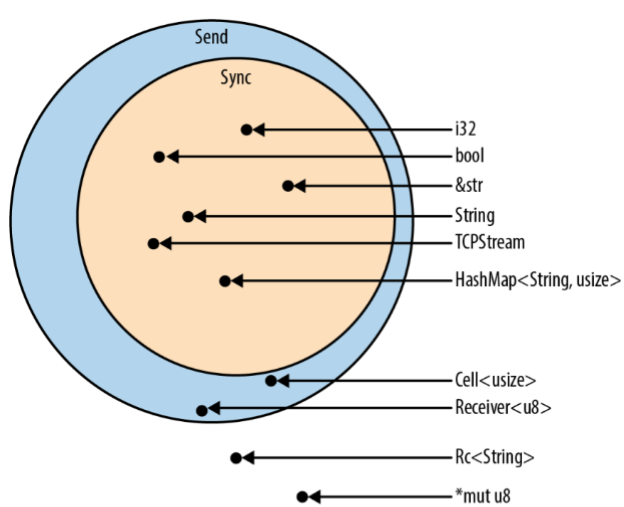
\includegraphics[width=\linewidth]{content/API_Programming/images/2026-04-28-12-10-05.png}
  \end{minipage}
\end{flushleft}


\begin{tcolorbox}
  \textbf{Note:}  \textbf{Send} riguarda il trasferimento, \textbf{Sync} la condivisione.
\end{tcolorbox}


È possibile creare thread solo se i dati catturati dalla funzione lambda che ne
descrive la computazione e il suo tipo di ritorno hanno il tratto \textbf{Send}, altrimenti
il compilatore genererà un errore.

In mancanza di questa garanzia, il borrow checker genera un errore di compilazione, rilevando la
propria impossibilità a garantire la correttezza di quanto si sta chiedendo di eseguire.


\begin{center}
  \begin{minipage}{0.45\linewidth}
    \begin{minted}[breaklines]{rust}
fn main() {
  let data1 = Rc::new(1);
  let data2 = data1.clone();

  println!("t0: {}", *data1);
  let jh = spawn(move || {
    println!("t1: {}", *data2);
  });

  jh.join().unwrap();
}
\end{minted}
  \end{minipage}%
  \hfill
  \begin{minipage}{0.45\linewidth}
    \centering
    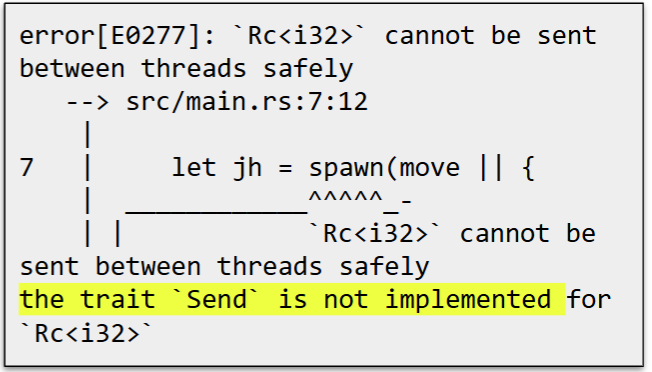
\includegraphics[width=\linewidth]{content/API_Programming/images/2026-04-28-12-16-27.png}
  \end{minipage}
\end{center}


\begin{table}[h!]
  \renewcommand{\arraystretch}{1.6}
  \centering
  \begin{tabular}{l l l l}
    \toprule
    \textbf{Tipo}     & \textbf{Send}         & \textbf{Sync}          & \textbf{Note}                             \\
    \midrule
    \texttt{Rc<T>}    & No                    & No                     & Conteggio dei riferimenti non thread-safe \\
    \texttt{Arc<T>}   & Sì                    & Sì, se lo è \texttt{T} & Conteggio dei riferimenti thread-safe     \\
    \texttt{Cell<T>}  & Dipende da \texttt{T} & No                     & Mutabilità interna                        \\
    \texttt{Mutex<T>} & Sì                    & Sì, se lo è \texttt{T} & Accesso protetto                          \\
    \bottomrule
  \end{tabular}
\end{table}


\section{Modello di concorrenza}
La libreria standard di Rust supporta \textbf{due modelli} base per la realizzazione di
programmi concorrenti

\begin{enumerate}
  \item La condivisione di dati basata su sincronizzazione degli accessi ad
        una \textbf{struttura dati condivisa}, a cui tutti i thread interessati possono
        accedere in lettura e scrittura.
        Tutti i thread possono leggere e scrivere in questa struttura dati.
  \item La condivisione di dati basata sullo \textbf{scambio di messaggi} che prevede
        uno o più mittenti ed un solo destinatario.
        Questa soluzione è più semplice e si adatta a meno situazioni rispetto alla prima.
        L'implementazine base è many-to-one, dove molti leggono e solo uno scrive.
\end{enumerate}

Sono inoltre disponibili librerie esterne che supportano ulteriori modelli:

\begin{itemize}
  \item La libreria \textbf{actix} supporta il modello degli attori
  \item La libreria \textbf{rayon} supporta il modello work stealing
  \item La libreria \textbf{crossbeam} permette la condivisione di
        dati memorizzati nello stack del thread genitore con i thread figli
\end{itemize}

\section{Condivisione dello stato}

Per poter condividere dati modificabili tra thread differenti, occorre disporre
di un qualche meccanismo che permetta, ad un solo thread alla volta, di
acquisire il permesso di modifica, questo lo svolgimento degli altri thread
che dovessero richiedere accesso alla stessa risorsa.


\paragraph{Mutex}
Il modo più semplice di ottenere questo comportamento è attraverso l'uso di un \textbf{mutex} -
MUTual EXclusion lock.
Costrutti di questo tipo sono offerti nativamente dai sistemi operativi e sono
riesportati in modo indipendente dalla piattaforma dalle librerie standard C++ e
Rust.

\paragraph{Lock e Unlock}

Gli oggetti nativi offerti dai sistemi operativi offrono, come minimo, due metodi: \verb|lock()|
e \verb|unlock()|.

\begin{itemize}
  \item Invocando, \verb|lock()|, un thread richiede il possesso del mutex: se questo non
        può essere garantito al momento, perché il mutex è in uso ad un altro thread,
        l'invocazione si blocca fino a che il mutex non è stato rilasciato
        dall'attuale possessore
  \item È lecito invocare \verb|unlock()| solo se il thread che lo esegue è
        l'attuale possessore del mutex
\end{itemize}


Entrambi i metodi \verb|lock()| e \verb|unlock()| includono una barriera di memoria.
Essa garantisce la visibilità delle operazioni eseguite fino a quel punto dagli
altri thread. Permette di imporre la dipendenza causale.

Sul piano pratico, occorre associare ad ogni risorsa condivisa un mutex che deve essere
\textbf{sempre} acquisito prima di fare accesso, sia in lettura che in scrittura, alla risorsa.


Nelle astrazioni base offerte dai sistemi operativi e nell'implementazione
offerta in C++, non c'è una corrispondenza sintattica tra un mutex e la
struttura dati che questo protegge. La relazione, in questi ambienti, è nella
mente, e nelle intenzioni, del programmatore.

Un mutex può, in linea di
principio, proteggere molte strutture diverse, ma riduce il grado di
parallelismo complessivo del programma.


\begin{center}
  \begin{minipage}{0.3\linewidth}
    \begin{minted}[breaklines]{rust}
std::list<int> l;
std::mutex m;
void add(int i){
  m.lock();
  l.push_back(i);
  m.unlock();
}
\end{minted}
  \end{minipage}%  
  \hfill
  \begin{minipage}{0.65\linewidth}
    \centering
    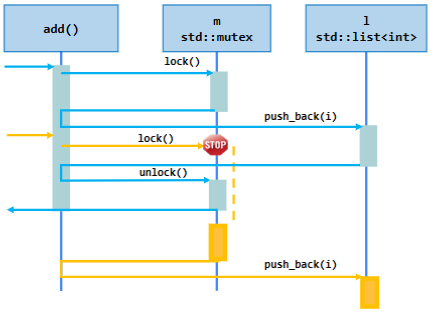
\includegraphics[width=0.5\linewidth]{content/API_Programming/images/2026-04-28-12-31-38.png}
  \end{minipage}
\end{center}


\section{Rilasciare i mutex}
Se un thread che è in possesso di un mutex termina, anche, ma non solo, per via
di un errore, senza rilasciare il mutex, si crea un problema.

\begin{itemize}
  \item I sistemi operativi tendono liberare il mutex
  \item Però, quale stato hanno le risorse che il mutex protegge?
\end{itemize}

Per evitare la situazione, nei linguaggi che lo supportano si ricorre al
paradigma RAII. Si incapsula l'acquisizione del lock nel costruttore di un
oggetto ``guardia'' e il suo rilascio nel distruttore. Si lega il ciclo di vita
dell'oggetto guardia al blocco di codice in cui occorre fare accesso al dato
protetto.


\section{Mutex in Rust}
L'accesso ad uno stato condiviso in Rust richiede l'utilizzo di \textbf{due blocchi} in cascata:

\begin{itemize}
  \item Il primo volto a permettere il possesso multiplo di una struttura dati
        in sola lettura da parte di più thread, realizzato mediante il costrutto std::
        \verb|sync::Arc<T>|
  \item Il secondo che consente l'acquisizione in lettura/scrittura della
        struttura dati, realizzato alternativamente mediante il costrutto
        \verb|std::sync::Mutex<T>|, con \verb|std::sync::RwLock<T>| oppure ricorrendo ai \textbf{tipi atomici}
\end{itemize}

Questa combinazione che prende spunto dal pattern RAII, permette di rendere
esplicito nella struttura del codice e nei pattern di accesso ai dati cosa sia
condiviso e impedisce di fatto l'accesso senza il corretto possesso del lock
relativo, permettendo al compilatore di bloccare ogni tentativo di accesso non
conforme.


\subsection{std::sync::Mutex<T>}

\begin{flushleft}
  \begin{minipage}{0.65\linewidth}
    \raggedright
    Un oggetto di tipo \verb|Mutex<T>| incapsula un dato di tipo \textbf{T} oltre al
    riferimento ad un mutex nativo del sistema operativo.

    L'unico modo per accedere al dato è invocare il metodo \verb|lock()|. Questo
    metodo restituisce un oggetto di tipo \verb|LockResult<MutexGuard<T>>| e resta
    bloccato fino a che non è stato possibile acquisire il mutex nativo. Se
    l'ultimo thread che ha acquisito il mutex fosse terminato prima di averlo
    rilasciato, il mutex si troverebbe nello stato avvelenato, e la risposta
    conterrebbe un errore.


    Se il metodo \verb|lock()| ha successo, la risposta contiene un \verb|MutexGuard<T>|,
    uno smart pointer.
    Tale oggetto implementa il tratto \verb|Deref<T>| e si comporta come uno
    smart-pointer. Dereferenziandolo, si ottiene un riferimento mutabile al
    dato T. Quando il MutexGuard<T> esce dallo scope, il mutex nativo viene
    rilasciato, permettendo ad altri thread di chiederne il possesso.


    Un valore di tipo \verb|MutexGuard<T>| deve restare in vita solo per il tempo
    strettamente necessario. Evitando I/O e computazioni lunghe mentre si
    possiede il lock.


    \begin{tcolorbox}
      \textbf{Note:} Se un thread panicasse, \textbf{poisoned} verrebbe settato.
    \end{tcolorbox}


  \end{minipage}%
  \hfill
  \begin{minipage}{0.3\linewidth}
    \centering
    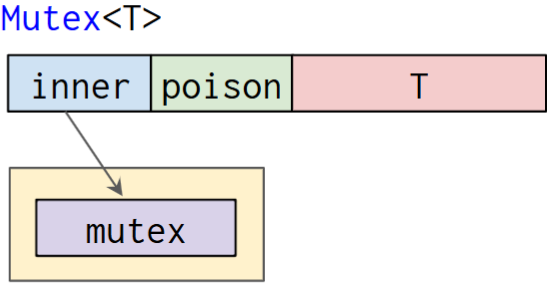
\includegraphics[width=\linewidth]{content/API_Programming/images/2026-04-28-12-45-09.png}
  \end{minipage}
\end{flushleft}


\begin{minted}[breaklines]{rust}
use std::sync::Mutex;
use std::sync::Arc;
use std::thread;

fn main(){
  let mut v: Vec<i32> = vec![];

  // la coda è all'italiana, onAvg è più efficeinte perché non 
  // c'è una sovrastruttura per mantenere l'ordine
  // ma questo può causare starvation
  let m = Mutex::new(v);

  // arc rende accessibile il dato a più proprietari, essendo thread safe
  // solitamente si passano strutture 
  let a = Arc::new(m);

  let a1 = a.clone();
  let a2 = a.clone();

  //due puntatori che conoscono il mutex

  let t1 = thread::spawn(move || {
    // il lock può essere avvelenato, devo gestire l'errore
    if let Ok(mut g) = a1.lock() {
      g.push(1);
      g.push(2);
      g.push(3);
    } // g esce di scope e rilascia il lock (unlock)
  });

  let t2 = thread::spawn(move || {
    if let Ok(mut g) = a2.lock() {
      g.push(4);
      g.push(5);
      //panic!("Errore irreversibile"); // il lock è avvelenato
      g.push(6);
    }
  });

  // t1.join().unwrap();
  // t2.join().unwrap();

  // riprendo il possesso del lock
  // println!("{:?}", a.lock().unwrap());

  if let Ok(_) = t1.join() {}
  if let Ok(_) = t2.join() {}

  if let Ok(v) = a.lock() {
    println!("{:?}", v);
  } else{
    println!("Il lock è avvelenato");
  }

  // possibili output: [1,2,3,4,5,6] oppure [4,5,6,1,2,3] 

}
\end{minted}

\begin{tcolorbox}
  \textbf{Note:} Il mutex è utilizzato se almeno uno deve scrivere, altrimenti è sufficiente utilizzare
  Arc<T> da solo.
  Se si vuole principalmente leggere, è meglio utilizzare RwLock<T> al posto di Mutex<T>.
\end{tcolorbox}



\subsection{std::sync::Arc<T>}


\begin{center}
  \begin{minipage}{0.65\linewidth}
    Un oggetto di tipo \textbf{Mutex} può avere un solo possesore. Per superare
    questo vincolo, lo si incapsula all'interno di un oggetto di tipo \verb|std::sync::Arc<T>|.

    \verb|Arc<T>| permette di condividere il possesso di un dato, allocandolo nello heap e
    mantenendo un conteggio dei riferimenti esistenti di tipo \textit{thread-safe}.

    È possibile duplicare un oggetto di questo tipo attraverso il metodo \verb|clone()|.
    Tale metodo si limita a duplicare il puntatore al blocco sullo heap,
    avendo cura di incrementare, in modo atomico, il contatore dei riferimenti
    associati al dato.
    Il dato clonato viene ceduto ad un thread specificando
    la parola-chiave move di fronte alla funzione lambda che ne descrive la
    computazione

  \end{minipage}%
  \hfill
  \begin{minipage}{0.3\linewidth}
    \centering
    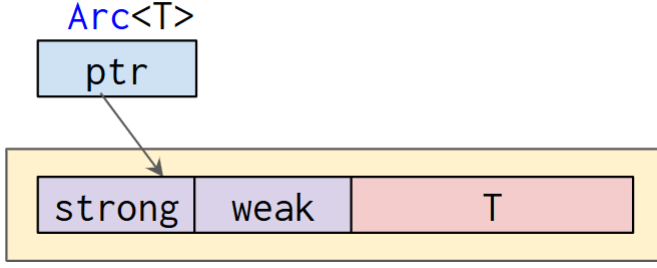
\includegraphics[width=\linewidth]{content/API_Programming/images/2026-04-28-12-55-39.png}
  \end{minipage}
\end{center}

\paragraph{Condivisione dello stato}

\begin{minted}[breaklines]{rust}
let shared_data = Arc::new(Mutex::new(Vec::new()));
let mut threads = vec![];
for (i in 1..10) {
  let mut data = shared_data.clone(); // duplicazione del possesso
  threads.push( thread::spawn( move || { // data è ceduto al thread
  let mut v = data.lock().unwrap(); // v è di tipo MutexGuard<T>
  v.push(i); // quando v esce dall scope
  }) ); // il lock viene rilasciato
}
for t in threads { t.join().unwrap(); } //v contiene i numeri da 1 a 9
\end{minted}

\begin{tcolorbox}
  \textbf{Note:} \textbf{Arc<Mutex<T>\>} = possesso condiviso + accesso mutabile protetto
\end{tcolorbox}



Se un thread viene creato mediante la primitiva \verb|std::thread::spawn()|, il
compilatore non può fare assunzioni sulla sua durata, di conseguenza, impedisce
l'utilizzo di riferimenti condivisi tra la funzione lambda del thread e la
funzione all'interno della quale il thread viene creato.

La libreria standard offre un ulteriore modo di creare un thread, tramite la
funzione \mintinline{rust}|std::thread::scope(|s: std::thread::Scope| {...})|.

Posso creare dei thread che possono durare meno della funzione scope stessa, a differenza
della primitiva spawn che si sa quando parte ma non quando finisce.
Questo permette di non aspettare le handle dei thread creati e di aspettare
se ogni thread ha finito la sua esecuzione.

Essa accetta come parametro una funzione lambda il cui compito è racchiudere l'intero ciclo di vita dei
thread creati al suo interno.
Il parametro s passato a tale funzione offre il metodo \verb|.spawn(...)| mediante
il quale è possibile creare nuovi thread.

Terminata l'esecuzione della funzione lambda, la funzione \verb|scope(...)| non
ritorna fino a che tutti i thread creati al suo interno non sono terminati.
Questo permette al borrow checker di considerare corretto l'uso di riferimenti a
variabili locali, dato che la loro durata sarà almeno pari a quella della
funzione \verb|scope(...)| e, di conseguenza, a quella dei thread creati al suo
interno.

Differenza chiave rispetto a \verb|thread::spawn( )|:
Con \verb|thread::scope(...)| il compilatore sa che i thread terminano prima dell'uscita dallo
scope




\begin{minted}[breaklines]{rust}
let mut v = vec![1, 2, 3];
let mut x = 0;
thread::scope(|s| {
  s.spawn(|| { // è lecito creare un riferimento a v
  println!("length: {}", v.len());
  });

  s.spawn(|| { // anche qui viene catturato &v
  for n in &v {println!("{n}"); }
  x += v[0]+v[2]; // x è catturata come &mut
  });
});
// Solo quando entrambi i thread saranno terminati si proseguirà
v.push(4); // non ci sono più riferimenti, si può modificare
assert_eq!(x, v.len());
\end{minted}


\subsection{std::sync::RwLock<T>}


\begin{center}
  \begin{minipage}{0.65\linewidth}
    Se gli accessi in lettura e in scrittura sono sbilanciati, può essere
    conveniente sostituire, alla \verb|struct Mutex<T>|, la \verb|struct RwLock<T>|.
    Questa offre il metodo \verb|read()| per accedere, in modo condiviso, in lettura ed il
    metodo \verb|write()| per accedere in modo esclusivo in scrittura
  \end{minipage}%
  \hfill
  \begin{minipage}{0.3\linewidth}
    \centering
    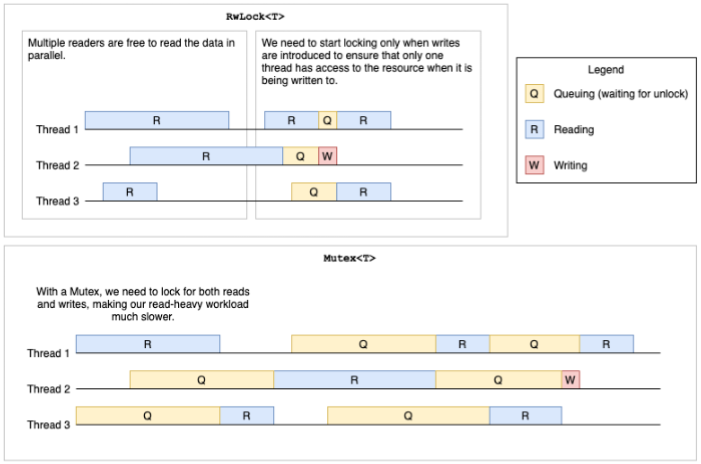
\includegraphics[width=\linewidth]{content/API_Programming/images/2026-04-28-14-21-14.png}
  \end{minipage}
\end{center}


\begin{center}
  \begin{minipage}{0.45\linewidth}

  \end{minipage}%
  \hfill
  \begin{minipage}{0.45\linewidth}
    \begin{minted}[breaklines]{rust}

\end{minted}
  \end{minipage}
\end{center}


\section{Tipi atomici}

È il tipo più elementare di Mutex, è pure meno costoso rispetto ad richiedere un lock.

Il modulo \verb|std::sync::atomic| mette a disposizione alcune strutture dati
che costituiscono primitive di comunicazione tra thread basate sul principio
della memoria condivisa. Esso offre versioni atomiche di valori booleani, numeri
interi con e senza segno e puntatori nativi.
Ciascun tipo è associato ad operazioni che, se usate correttamente, permettono
di sincronizzare gli aggiornamenti di tali valori tra thread differenti.


Accanto alle operazioni di lettura e scrittura con associata barriera di memoria,
questi tipi offrono funzionalità di tipo Read-Modify-Write:

\begin{center}
  \verb|swap(...)|, \verb|compare_exchange(...)|, \verb|fetch_add(...)|, \verb|fetch_update(...)|
\end{center}

Ciascuna di queste operazioni riceve come parametro esplicito il tipo di barriera di memoria da
applicare per la fase di lettura e per quella di scrittura.


\begin{tcolorbox}
  \textbf{Note:} prima di utilizzare i tipi atomici, bisogna mangairne di pasta, pensa ad
  imparare gli altri.
\end{tcolorbox}


Sebbene siano tutti thread-safe, implementano il tratto \textit{Sync}, non offrono
meccanismi di condivisione esplicita. Come tutti i valori in Rust, sono
soggetti alla regola del possessore unico. Per permettere a più thread di
accedere al loro valore, è comune incapsularli all'interno di un elemento di
tipo \verb|Arc<T>| oppure dichiararli come variabili globali, attraverso la parola
chiave static.


In modo analogo a \verb|Cell<T>|, implementano il meccanismo di
mutabilità interna. Poiché le operazioni di modifica sono garantite essere
thread-safe, i metodi che ne modificano il contenuto richiedono solo un accesso
condiviso (\verb|\&self|) e non un accesso esclusivo(\verb|\&mut self|)



\begin{tcolorbox}
  \textbf{Note:} I tipi atomici sono potenti ma più difficili da usare
  correttamente rispetto ai lock Richiedono particolare attenzione
  all'ordinamento della memoria
\end{tcolorbox}

\begin{minted}[breaklines]{rust}
use std::sync::Arc;
use std::sync::atomic::{AtomicUsize, Ordering};
use std::{hint, thread};

fn main() {
  let spinlock = Arc::new(AtomicUsize::new(1));
  let spinlock_clone = Arc::clone(&spinlock);
  
  let thread = thread::spawn(move|| {
    spinlock_clone.store(0, Ordering::Release);
  });
  // Attendi
  while spinlock.load(Ordering::Acquire) != 0 {
    hint::spin_loop();
  }

  thread.join().unwrap();
}
\end{minted}












